% !TeX program = xelatex
% 4.2.1 指数函数的概念 · 本节图形（pgfplots 图集）
% 编译：xelatex 本节图形_pgfplots.tex（连续两遍）
% 说明：下面每个 tikzpicture 均可直接复制进 beamer 的 frame 中使用。
\documentclass[11pt]{ctexart}

\usepackage{amsmath,amssymb}
\usepackage{pgfplots}
\pgfplotsset{compat=1.18}
\usepackage{float}
\usepackage{caption}

% ---- 思源字体 ----
\setCJKmainfont{Source Han Serif SC}[BoldFont={Source Han Serif SC Bold}]
\setCJKsansfont{Source Han Sans SC}[BoldFont={Source Han Sans SC Bold}]

% ---- 配色 ----
\definecolor{mainblue}{RGB}{23,103,171}
\definecolor{dotpink}{RGB}{214,60,120}

% 散点 + 趋势线通用样式（x 为距 2001 年的偏移年，刻度映射回年份）
\pgfplotsset{
  scenic/.style={
    width=7.2cm, height=5.6cm,
    xmin=-0.7, xmax=14.7, ymin=300, ymax=1300,
    xtick={0,2,4,6,8,10,12,14},
    xticklabels={2001,2003,2005,2007,2009,2011,2013,2015},
    ytick={300,500,700,900,1100,1300},
    xlabel={时间/年}, ylabel={人次/万次},
    axis lines=left,
    label style={font=\small},
    tick label style={font=\footnotesize,
      /pgf/number format/1000 sep={}},
    enlargelimits=0.03,
  },
}

\begin{document}

\section*{图 4.2-1\quad A 地景区游客人次（近似线性增长）}
\begin{figure}[H]
  \centering
  \begin{tikzpicture}
    \begin{axis}[scenic]
      % 表 4.2-1 中 A 地景区人次（万次），x 为距 2001 年的年数
      \addplot[only marks, mark=*, dotpink, mark size=2.2pt] coordinates {
        (0,600) (1,609) (2,620) (3,631) (4,641)
        (5,650) (6,661) (7,671) (8,681) (9,691)
        (10,702) (11,711) (12,721) (13,732) (14,743)
      };
      % 线性趋势线：年增加量约 10 万次
      \addplot[mainblue, dashed, thick, domain=0:14]
        {600 + 10.21*x};
    \end{axis}
  \end{tikzpicture}
  \caption*{图 4.2-1}
\end{figure}

\section*{图 4.2-2\quad B 地景区游客人次（指数增长）}
\begin{figure}[H]
  \centering
  \begin{tikzpicture}
    \begin{axis}[scenic]
      % 表 4.2-1 中 B 地景区人次（万次），x 为距 2001 年的年数
      \addplot[only marks, mark=*, dotpink, mark size=2.2pt] coordinates {
        (0,278) (1,309) (2,344) (3,383) (4,427)
        (5,475) (6,528) (7,588) (8,655) (9,729)
        (10,811) (11,903) (12,1005) (13,1118) (14,1244)
      };
      % 指数增长曲线：y = 278 × 1.11^x
      \addplot[mainblue, dashed, thick, domain=0:14]
        {278*1.11^x};
    \end{axis}
  \end{tikzpicture}
  \caption*{图 4.2-2}
\end{figure}

\section*{图 4.2-3\quad 例 2(1) A、B 两地旅游收入对比}
\begin{figure}[H]
  \centering
  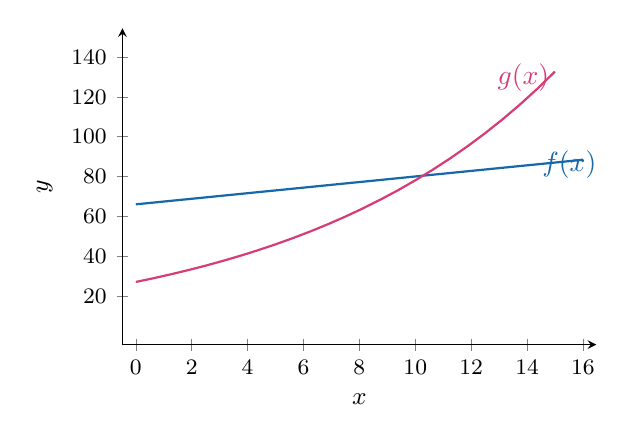
\begin{tikzpicture}
    \begin{axis}[
      width=7.6cm, height=5.6cm,
      xmin=0, xmax=16, ymin=0, ymax=150,
      xtick={0,2,4,6,8,10,12,14,16}, ytick={20,40,60,80,100,120,140},
      xlabel={$x$}, ylabel={$y$},
      axis lines=left,
      label style={font=\small},
      tick label style={font=\footnotesize},
      enlargelimits=0.03,
    ]
      % f(x)：A 地收入，近似直线缓升
      \addplot[mainblue, thick, domain=0:16] {66 + 1.4*x};
      \node[mainblue, anchor=west] at (axis cs:14.2,86) {$f(x)$};
      % g(x)：B 地收入，指数上凹增长，交点约 x≈10.22
      \addplot[dotpink, thick, domain=0:15] {27*1.112^x};
      \node[dotpink, anchor=south west] at (axis cs:12.6,118) {$g(x)$};
    \end{axis}
  \end{tikzpicture}
  \caption*{图 4.2-3}
\end{figure}

\section*{练习 1\quad 四个备选图象}
\begin{figure}[H]
  \centering
  \pgfplotsset{
    opt/.style={
      width=3.3cm, height=3.3cm,
      axis lines=middle, axis equal,
      xtick=\empty, ytick=\empty,
      xmin=-2, xmax=2, ymin=-2.5, ymax=2.5,
      every axis plot/.append style={mainblue, thick},
      samples=100,
    },
  }
  \begin{minipage}[t]{0.24\textwidth}
    \centering
    \begin{tikzpicture}
      \begin{axis}[opt]
        \addplot[domain=-1.6:1.8] {-x+1.3};
        \node at (axis cs:-0.15,-0.25) {$O$};
      \end{axis}
    \end{tikzpicture}\\[2pt]
    (A)
  \end{minipage}
  \begin{minipage}[t]{0.24\textwidth}
    \centering
    \begin{tikzpicture}
      \begin{axis}[opt]
        \addplot[domain=-1.8:1.8] {x^2-2};
        \node at (axis cs:-0.15,-0.25) {$O$};
      \end{axis}
    \end{tikzpicture}\\[2pt]
    (B)
  \end{minipage}
  \begin{minipage}[t]{0.24\textwidth}
    \centering
    \begin{tikzpicture}
      \begin{axis}[opt]
        \addplot[domain=-2:1.7] {2^x};
        \node at (axis cs:-0.15,-0.25) {$O$};
      \end{axis}
    \end{tikzpicture}\\[2pt]
    (C)
  \end{minipage}
  \begin{minipage}[t]{0.24\textwidth}
    \centering
    \begin{tikzpicture}
      \begin{axis}[opt]
        \addplot[domain=-1.5:1.5] {x^3};
        \node at (axis cs:-0.15,-0.25) {$O$};
      \end{axis}
    \end{tikzpicture}\\[2pt]
    (D)
  \end{minipage}
\end{figure}

\end{document}
